\documentclass{article}

% --- Math Packages ---
\usepackage{amsmath}
\usepackage{amssymb}
\usepackage{amsfonts}

% --- Typography and Layout ---
\usepackage[margin=1in]{geometry}
\usepackage{microtype}

% --- Figures and Tables ---
\usepackage{graphicx}
\usepackage{subcaption}
\usepackage{booktabs}

% --- Referencing and Links ---
\usepackage{hyperref}
\usepackage{cleveref}

% --- Hyperref Configuration ---
\hypersetup{
  colorlinks=true,
  linkcolor=blue,
  filecolor=magenta,
  urlcolor=cyan,
  pdftitle={A Tutorial on Digit Recurrence Algorithms for Division and Square Root},
  pdfpagemode=FullScreen,
}

% --- Custom Commands and Operators ---
% Custom operator for integer part
\DeclareMathOperator{\Int}{Int}

% --- Document Metadata ---
\title{A Tutorial on Digit Recurrence Algorithms\\
for Division and Square Root}
\author{Joonsang Yoon}
\date{\today}

\begin{document}

\maketitle

\begin{abstract}
  Digit recurrence algorithms, particularly the SRT (Sweeney, Robertson, and Tocher) family, form the backbone of high-speed division and square root units in digital computers.
  They achieve high performance by employing a redundant number system for the result digits.
  This core principle of redundancy introduces tolerance for imprecision, allowing the critical digit selection step to be performed with fast, truncated estimates of the internal state, thereby avoiding the performance bottleneck of full-width carry-propagating additions.
  This paper provides a comprehensive tutorial on the theory and practice of these algorithms.
  We present a step-by-step derivation of the fundamental recurrence relations for both division and square root.
  The tutorial meticulously explains how to establish the convergence conditions and then guides the reader through the complete design process for the digit selection logic.
  To ground the theory in practice, we develop detailed Radix-2 and Radix-4 examples, demonstrating how to determine key design parameters and derive the final selection logic from first principles.
\end{abstract}

\section{Introduction}
\label{sec:introduction}
Division and square root are fundamental arithmetic operations in modern microprocessors, essential for a wide range of applications in scientific computing, signal processing, and graphics.
Unlike addition and multiplication, which can be implemented with relatively straightforward combinatorial logic, division and square root are inherently iterative.
The most prevalent and efficient hardware methods for these operations are digit recurrence algorithms.

The core idea of a digit recurrence algorithm is to compute the result (quotient or square root) one digit at a time, from most significant to least significant.
Each iteration involves two main steps: selecting a new digit of the result and calculating a new partial remainder, or \emph{residual}.
The performance of the entire algorithm hinges on the speed of this iterative loop.
A naive implementation faces a critical bottleneck in the digit selection step.
To select a correct digit, one must compare the current residual against multiples of the divisor (or partial root).
This comparison requires the precise value of the residual, which is updated in every cycle.
Calculating this precise value would necessitate a full-width, carry-propagating addition, making the loop unacceptably slow.

The SRT family of algorithms, named after their independent inventors Sweeney, Robertson, and Tocher, provides an elegant solution to this bottleneck.
The key innovation is the use of a \emph{redundant digit set} for the result.
For example, in Radix-2, instead of the standard digits $\{0, 1\}$, a redundant set such as $\{-1, 0, 1\}$ is used.
This redundancy relaxes the constraints on digit selection, creating an overlap between the valid selection regions for adjacent digits.
This overlap is the crucial feature that enables high performance: because the regions overlap, a correct digit can be chosen using a low-precision, truncated estimate of the residual.
This eliminates the need for a slow, full-width addition in the critical path.
The iterative loop can thus be made very fast, typically limited only by a short carry-propagate addition on a few most-significant bits and a small lookup table.

This paper serves as a tutorial on the design and analysis of digit recurrence algorithms, providing a thorough and clear exposition of their mathematical foundations.
The structure of the paper is as follows:
\begin{itemize}
  \item \cref{sec:redundancy} introduces the concept of redundant digit sets and the redundancy factor $\rho$, the parameter that quantifies the overlap essential to these algorithms.
  \item \cref{sec:division} provides a complete derivation of the digit recurrence algorithm for division. We establish the residual recurrence, the containment condition, and the digit selection intervals, then show how to design practical selection logic using truncated operands for Radix-2 and Radix-4.
  \item \cref{sec:sqrt} extends the methodology to the square root operation. We derive the corresponding recurrence relations and selection intervals, highlighting the similarities and key differences compared to division, and again provide detailed Radix-2 and Radix-4 design examples.
  \item \cref{sec:conclusion} summarizes the key principles and design trade-offs discussed throughout the paper.
\end{itemize}

\section{Redundancy in Digit Sets}
\label{sec:redundancy}
The cornerstone of high-speed digit recurrence algorithms is the use of a redundant number system for the digits of the result.
Instead of a standard non-redundant set for radix $B$, such as $\{0, 1, \dots, B-1\}$, these algorithms employ a symmetric, redundant digit set.

At each step $j$ of the algorithm, the selected digit ($q_{j+1}$ for division or $s_{j+1}$ for square root) is chosen from the set:
\begin{equation}
  \label{eq:redundancy:digit_set}
  q_{j+1}, s_{j+1} \in \{-a, -a+1, \dots, a-1, a\}
\end{equation}
where $a$ is an integer representing the largest possible digit magnitude.
The degree of redundancy is quantified by the \emph{redundancy factor}, $\rho$, defined as the ratio of the largest digit in the redundant set to the largest digit in a non-redundant set:
\begin{equation}
  \label{eq:redundancy:rho_def}
  \rho = \frac{a}{B-1}
\end{equation}
The fundamental requirement for a high-speed SRT-style algorithm is that this redundancy factor must be greater than one-half:
\begin{equation}
  \rho > \frac{1}{2}
\end{equation}
This condition is critical because it guarantees that the \emph{selection intervals} for adjacent digits overlap.
As we will derive in \cref{sec:division}, the choice of a digit $k$ is valid only for a certain range of residual values.
The condition $\rho > 1/2$ ensures that the valid range for selecting digit $k$ and the valid range for selecting digit $k+1$ have a non-empty intersection.
This overlap means there are values of the residual for which either choice is correct.
It is precisely this flexibility that allows the digit selection to be based on a fast, truncated estimate of the residual, rather than its exact, slowly-computed value.
A non-redundant system corresponds to $\rho = 1/2$, where selection intervals meet at precise boundaries, demanding an exact comparison.

The constraints on the digit magnitude $a$ are a direct consequence of the required range for $\rho$.
For a practical and efficient implementation, $\rho$ is bounded as:
\begin{equation}
  \label{eq:redundancy:rho_range}
  \frac{1}{2} < \rho \leq 1
\end{equation}
Substituting the definition of $\rho$ from \cref{eq:redundancy:rho_def} into this inequality yields the required range for $a$:
\begin{equation}
  \label{eq:redundancy:a_range}
  \frac{B-1}{2} < a \leq B-1
\end{equation}
The lower bound, $a > (B-1)/2$, is the mathematical requirement to ensure $\rho > 1/2$ and thus guarantee the essential overlap.
The upper bound, $a \leq B-1$, is a practical hardware constraint.
While a larger $a$ provides more redundancy, choosing $a > B-1$ complicates the logic needed to form the term $q_{j+1}D$ in the recurrence, offering diminishing returns for the added complexity.
A choice of $a = B-1$ (where $\rho = 1$) is termed ``maximally redundant,'' while choices of $a$ closer to $(B-1)/2$ (where $\rho \to 1/2$) are ``minimally redundant.''

\section{Division by Digit Recurrence}
\label{sec:division}
We begin by developing the algorithm for division.
The fundamental relationship is:
\begin{equation}
  \label{eq:division:relation}
  N = D Q + R
\end{equation}
where $N$ is the dividend, $D$ is the divisor, $Q$ is the quotient, and $R$ is the final remainder.
For fractional arithmetic, it is standard practice to normalize the operands.
We assume the following ranges:
\begin{align*}
  N &\in \left[\frac{1}{4}, \frac{1}{2}\right) && \text{(Dividend)} \\
  D &\in \left[\frac{1}{2}, 1\right) && \text{(Divisor)}
\end{align*}
These ranges guarantee that the quotient $Q$ is also in a predictable range, preventing overflow and simplifying the algorithm:
\begin{equation}
  \label{eq:division:q_range}
  Q \in \left(\frac{N_{\min}}{D_{\max}}, \frac{N_{\max}}{D_{\min}}\right) = \left(\frac{1/4}{1}, \frac{1/2}{1/2}\right) = \left(\frac{1}{4}, 1\right)
\end{equation}

The quotient $Q$ is computed iteratively over $n$ steps, where $j = 0, 1, \dots, n-1$.
Let $Q_j$ be the quotient estimate after $j$ digits ($q_1, \dots, q_j$) have been determined.
The quotient is refined at each step by adding a new term:
\begin{equation}
  \label{eq:division:quotient_recurrence}
  Q_{j+1} = Q_j + q_{j+1} B^{-(j+1)}
\end{equation}
Unfolding this recurrence shows the composition of the quotient at step $j$:
\begin{equation}
  \label{eq:division:quotient_unfold}
  \text{At step } j, \quad Q_{j+1} = Q_0 + \sum_{i=0}^{j} q_{i+1} B^{-(i+1)}
\end{equation}
After $n$ iterations, the final quotient is computed to the desired precision:
\begin{equation}
  \label{eq:division:quotient_final}
  \text{At step } j = n-1, \quad Q_n = Q_0 + \sum_{i=0}^{n-1} q_{i+1} B^{-(i+1)} = Q
\end{equation}
The core of the algorithm is ensuring that the process converges to the true quotient.
At any step $j$, the error in the current approximation $Q_{j+1}$ is given by:
\begin{equation}
  \label{eq:division:error_def}
  \varepsilon_{j+1} = \frac{N}{D} - Q_{j+1} = \sum_{i=j+1}^{\infty} q_{i+1} B^{-(i+1)}
\end{equation}
The magnitude of this error is bounded by the largest possible value of the remaining undiscovered digits.
Using the digit bound $a$:
\begin{equation}
  \label{eq:division:error_sum}
  \left| \sum_{i=j+1}^{\infty} q_{i+1} B^{-(i+1)} \right| \leq \sum_{i=j+1}^{\infty} a B^{-(i+1)} = a B^{-(j+2)} \sum_{k=0}^{\infty} B^{-k} = a B^{-(j+2)} \frac{1}{1-B^{-1}} = \frac{a}{B-1} B^{-(j+1)}
\end{equation}
This gives the fundamental error bound in terms of the redundancy factor $\rho$:
\begin{equation}
  \label{eq:division:error_bound}
  \left| \varepsilon_{j+1} \right| \leq \rho B^{-(j+1)}
\end{equation}
Substituting the definition of the error, we get:
\begin{equation}
  \label{eq:division:error_bound_sub}
  \left| \frac{N}{D} - Q_{j+1} \right| \leq \rho B^{-(j+1)}
\end{equation}
To work with integer-like quantities in hardware, we define a scaled residual, $R_{j+1}$.
Multiplying by $D$ and scaling by $B^{j+1}$ gives:
\begin{equation}
  \label{eq:division:scaled_error}
  \left| B^{j+1} (N - D Q_{j+1}) \right| \leq \rho D
\end{equation}
We define the scaled residual at the end of step $j$ as:
\begin{equation}
  \label{eq:division:residual_def}
  R_{j+1} = B^{j+1} (N - D Q_{j+1})
\end{equation}
This leads to the crucial \emph{containment condition}: the residual must always be bounded by a multiple of the divisor.
\begin{equation}
  \label{eq:division:containment}
  \left| R_{j+1} \right| \leq \rho D
\end{equation}
The final, unscaled remainder $R$ is related to the final residual $R_n$ by:
\begin{equation}
  \label{eq:division:final_remainder}
  \text{At step } j = n-1, \quad R_n = B^n (N - D Q_n) = B^n R
\end{equation}
To implement the algorithm, we need an iterative way to compute $R_{j+1}$ from $R_j$.
We derive this recurrence from its definition in~\cref{eq:division:residual_def}:
\begin{align*}
  R_{j+1} &= B^{j+1} (N - D Q_{j+1}) && \text{Definition of } R_{j+1} \\
  &= B^{j+1} \left(N - D \left(Q_j + q_{j+1} B^{-(j+1)}\right)\right) && \text{Using \cref{eq:division:quotient_recurrence}} \\
  &= B^{j+1} (N - D Q_j) - B^{j+1} D q_{j+1} B^{-(j+1)} && \text{Distributing } D \\
  &= B \left(B^j (N - D Q_j)\right) - q_{j+1} D && \text{Simplifying} \\
  &= B R_j - q_{j+1} D && \text{Using the definition of } R_j
\end{align*}
This gives the central recurrence relation for division:
\begin{equation}
  \label{eq:division:residual_recurrence}
  R_{j+1} = B R_j - q_{j+1} D
\end{equation}
At each step $j$, the algorithm performs two main tasks: (1) select a digit $q_{j+1}$ based on the current residual $R_j$ and the divisor $D$, and (2) compute the next residual $R_{j+1}$ using this recurrence.
The selection of $q_{j+1}$ must be done such that the next residual $R_{j+1}$ satisfies the containment condition in~\cref{eq:division:containment}.

\subsection{Selection Intervals for a Positive Divisor}
\label{ssec:division:pos_divisor}
For a positive divisor, $D \in \left[\frac{1}{2}, 1\right)$, the containment condition from~\cref{eq:division:containment} is:
\begin{equation}
  \label{eq:division:containment_pos}
  \left| R_{j+1} \right| \leq \rho D \implies -\rho D \leq R_{j+1} \leq \rho D
\end{equation}
We substitute the recurrence relation from~\cref{eq:division:residual_recurrence} into this inequality:
\begin{equation}
  \label{eq:division:selection_sub_pos}
  -\rho D \leq B R_j - q_{j+1} D \leq \rho D
\end{equation}
To find the condition that $B R_j$ must satisfy to select a particular digit $q_{j+1}$, we add $q_{j+1} D$ to all parts of the inequality:
\begin{equation}
  \label{eq:division:selection_interval_pos}
  (q_{j+1} - \rho) D \leq B R_j \leq (q_{j+1} + \rho) D
\end{equation}
This equation defines a selection interval for each possible digit $q_{j+1}$.
The goal of the digit selection logic is to determine which interval the shifted residual $B R_j$ falls into.
The fact that $\rho > 1/2$ ensures these intervals overlap, making the selection robust to small errors.

\subsection{Selection Intervals for a Negative Divisor}
\label{ssec:division:neg_divisor}
For a negative divisor, $D \in \left[-1, -\frac{1}{2}\right)$, the magnitude is $|D| = -D$.
The containment condition is still based on the magnitude:
\begin{equation}
  \label{eq:division:containment_neg_mag}
  \left| R_{j+1} \right| \leq \rho |D| \implies \left| R_{j+1} \right| \leq -\rho D
\end{equation}
This expands to:
\begin{equation}
  \label{eq:division:containment_neg}
  \rho D \leq R_{j+1} \leq -\rho D
\end{equation}
Substituting the recurrence relation from~\cref{eq:division:residual_recurrence}:
\begin{equation}
  \label{eq:division:selection_sub_neg}
  \rho D \leq B R_j - q_{j+1} D \leq -\rho D
\end{equation}
Adding $q_{j+1} D$ yields the selection interval:
\begin{equation}
  \label{eq:division:selection_interval_neg}
  (q_{j+1} + \rho) D \leq B R_j \leq (q_{j+1} - \rho) D
\end{equation}

\subsection{Initialization}
\label{ssec:division:init}
The first step of the algorithm ($j = 0$) requires initial values for the quotient approximation, $Q_0$, and the residual, $R_0$.
These values must be chosen such that the first shifted residual, $B R_0$, falls within a valid selection region for the first quotient digit, $q_1$.
This ensures the recurrence can start correctly and that the subsequent residual, $R_1$, will satisfy the containment condition.

A common and robust initialization strategy is to set the initial quotient approximation to $Q_0 = 0$ and the initial residual to $R_0 = N / B$.
This choice has the convenient property that the first shifted residual is simply the dividend itself:
\begin{equation}
  \label{eq:division:init_br0}
  B R_0 = B \left(\frac{N}{B}\right) = N
\end{equation}
With the assumed operand ranges, for a positive divisor $D \in \left[\frac{1}{2}, 1\right)$, the dividend is $N \in \left[\frac{1}{4}, \frac{1}{2}\right)$, so the shifted residual $B R_0$ is also in the range $\left[\frac{1}{4}, \frac{1}{2}\right)$.

To verify this initialization, we must show that the range of $B R_0$ is fully covered by the union of the selection intervals for $q_1$, as defined in \cref{eq:division:selection_interval_pos} for a positive divisor.
The selection condition for $q_1$ is:
\begin{equation}
  \label{eq:division:init_selection}
  (q_1 - \rho) D \leq B R_0 \leq (q_1 + \rho) D
\end{equation}
Since $B R_0$ is positive, we only need to check the intervals for non-negative digits ($q_1 \in \{0, 1, \dots, a\}$).

In the Radix-2 case ($B = 2, \rho = 1$), the shifted residual range is $2 R_0 = N \in \left[\frac{1}{4}, \frac{1}{2}\right)$.
We check the selection intervals for $q_1 = 0$ and $q_1 = 1$:
\begin{itemize}
    \item For $q_1 = 1$: The interval is $[(1-1)D, (1+1)D] = [0, 2D]$.
    \item For $q_1 = 0$: The interval is $[(0-1)D, (0+1)D] = [-D, D]$.
\end{itemize}
The union of these intervals is $[-D, 2D]$.
For any $D \in \left[\frac{1}{2}, 1\right)$, this union covers at least $\left[-\frac{1}{2}, 1\right]$.
This range safely contains the required range of $2 R_0 \in \left[\frac{1}{4}, \frac{1}{2}\right)$, so the initialization is valid.

In the Radix-4 case ($B = 4, \rho = 2/3$), the shifted residual range is $4 R_0 = N \in \left[\frac{1}{4}, \frac{1}{2}\right)$.
We check the intervals for $q_1 \in \{0, 1, 2\}$:
\begin{itemize}
    \item For $q_1 = 2$: The interval is $\left[\left(2-\frac{2}{3}\right)D, \left(2+\frac{2}{3}\right)D\right] = \left[\frac{4}{3}D, \frac{8}{3}D\right]$.
    \item For $q_1 = 1$: The interval is $\left[\left(1-\frac{2}{3}\right)D, \left(1+\frac{2}{3}\right)D\right] = \left[\frac{1}{3}D, \frac{5}{3}D\right]$.
    \item For $q_1 = 0$: The interval is $\left[\left(0-\frac{2}{3}\right)D, \left(0+\frac{2}{3}\right)D\right] = \left[-\frac{2}{3}D, \frac{2}{3}D\right]$.
\end{itemize}
The union of these intervals is $\left[-\frac{2}{3}D, \frac{8}{3}D\right]$.
For any $D \in \left[\frac{1}{2}, 1\right)$, this union covers at least $\left[-\frac{1}{3}, \frac{4}{3}\right]$.
This range safely contains the required range of $4 R_0 \in \left[\frac{1}{4}, \frac{1}{2}\right)$, confirming the initialization is also valid for the Radix-4 case.

For a negative divisor, the analysis is analogous using the selection intervals from \cref{eq:division:selection_interval_neg}.
The principle of ensuring the initial shifted residual falls within the union of valid selection regions remains the same.

\subsection{Example: Radix-2 SRT Division}
\label{ssec:division:radix2}
Let's consider the simplest and most common case: Radix-2 ($B = 2$) with a maximally redundant digit set $\{-1, 0, 1\}$, which means we choose $a = 1$.
The redundancy factor is:
\begin{equation}
  \label{eq:division:radix2_rho}
  \rho = \frac{a}{B-1} = \frac{1}{2-1} = 1
\end{equation}

\subsubsection{Positive Divisor}
\label{sssec:division:radix2_pos}
With $\rho = 1$ and $B = 2$, the selection intervals from~\cref{eq:division:selection_interval_pos} become:
\begin{equation}
  \label{eq:division:radix2_intervals_pos}
  q_{j+1} =
  \begin{cases}
    1  & \text{if } 0 \leq 2 R_j \leq 2 D \\
    0  & \text{if } -D \leq 2 R_j \leq D \\
    -1 & \text{if } -2 D \leq 2 R_j \leq 0
  \end{cases}
\end{equation}
These intervals overlap.
For example, if $2R_j = 0.2D$, both $q_{j+1} = 1$ and $q_{j+1} = 0$ are valid choices.
This overlap is what allows for a simplified implementation.

In hardware, the residual $R_j$ is typically kept in carry-save form to avoid slow carry propagation in the main loop.
To perform the comparisons in the selection logic, we would need to compute the full value of $2R_j$, which requires a fast adder.
To avoid this, we compute an estimate of $2R_j$ by summing only a few of its most significant bits.

Let the full-precision shifted residual be $2 R_j = r_{j,2\ldots0}.r_{j,-1\ldots-\infty}$.
This value is the sum of two bit-vectors in carry-save representation:
$Y_j = y_{j,2\ldots0}.y_{j,-1\ldots-\infty}$ and $Z_j = z_{j,2\ldots0}.z_{j,-1\ldots-\infty}$.
\begin{equation}
  \label{eq:division:radix2_cs_sum}
  r_{j,2\ldots0}.r_{j,-1\ldots-\infty} = y_{j,2\ldots0}.y_{j,-1\ldots-\infty} + z_{j,2\ldots0}.z_{j,-1\ldots-\infty}
\end{equation}
We form a truncated estimate $t_j$ by adding the top bits of $Y_j$ and $Z_j$ using a small carry-propagate adder (CPA).
Let's say we use $\alpha$ fractional bits.
\begin{equation}
  \label{eq:division:radix2_trunc_sum}
  t_{j,2\ldots0}.t_{j,-1\ldots-\alpha} = y_{j,2\ldots0}.y_{j,-1\ldots-\alpha} + z_{j,2\ldots0}.z_{j,-1\ldots-\alpha}
\end{equation}
This truncation introduces a one-sided error.
The sum of the truncated parts is less than or equal to the true sum.
\begin{equation}
  \label{eq:division:radix2_trunc_error}
  0 \leq 2 R_j - t_{j,2\ldots0}.t_{j,-1\ldots-\alpha} < 2 \cdot 2^{-\alpha} = 2^{-(\alpha-1)}
\end{equation}
Similarly, we use a truncated version of the divisor $D$, using its first $\beta$ fractional bits.
We define integer-valued estimates for use in a simple lookup table (PLA):
\begin{align}
  \label{eq:division:radix2_tau_def}
  \tau_j &= \Int(2^\alpha \cdot t_{j,2\ldots0}.t_{j,-1\ldots-\alpha}) \in \left\{-2^{\alpha+2}, \dots, 2^{\alpha+2}-1\right\} && (\tau_j \leq 2^{\alpha+1} R_j < \tau_j + 2) \\
  \label{eq:division:radix2_delta_def}
  \delta &= \Int(2^\beta \cdot 0.1d_{j,-2\ldots-\beta}) \in \left\{2^{\beta-1}, \dots, 2^\beta-1\right\} && (\delta \leq 2^\beta D < \delta + 1)
\end{align}
The selection logic must choose a digit $k \in \{-1, 0, 1\}$ based on $\tau_j$ and $\delta$.

To ensure a correct digit can be selected using the truncated estimates, the selection regions must have sufficient overlap to absorb the uncertainty introduced by truncation.
This is formalized by the \emph{continuity condition}.
Let $L_k(D) = (k-\rho)D$ and $U_k(D) = (k+\rho)D$ be the lower and upper bounds of the selection interval for digit $k$.
The condition requires that for any adjacent digits $k$ and $k-1$, the region for $k-1$ must overlap with the region for $k$ even under the worst-case truncation errors.
Specifically, the minimum possible value of the upper bound for digit $k-1$ must be greater than or equal to the maximum possible value of the lower bound for digit $k$:
\begin{equation}
  \label{eq:division:continuity_condition}
  \min(U_{k-1, \text{trunc}}) \geq \max(L_{k, \text{trunc}})
\end{equation}
To evaluate this, we must find the extrema of the bounds over the uncertainty intervals of $D$ and $2R_j$.
The truncation of the residual introduces a one-sided error of up to $2^{-(\alpha-1)}$, which lowers the minimum value of the upper bound.
The truncation of the divisor means $D \in \left[2^{-\beta} \delta, 2^{-\beta} (\delta + 1)\right)$.
This leads to the following expressions for the truncated bounds (assuming positive coefficients for $D$):
\begin{align}
  \label{eq:division:continuity_uk}
  \min(U_{k-1, \text{trunc}}) &= \min_{D}(U_{k-1}(D)) - 2^{-(\alpha-1)} = (k - 1 + \rho) (2^{-\beta} \delta) - 2^{-(\alpha-1)} \\
  \label{eq:division:continuity_lk}
  \max(L_{k, \text{trunc}}) &= \max_{D}(L_{k}(D)) = (k - \rho) (2^{-\beta} (\delta + 1))
\end{align}
Substituting these into the continuity condition gives the inequality that must be solved to find the required precision parameters $\alpha$ and $\beta$.
For negative coefficients, the roles of $\delta$ and $\delta+1$ are swapped.
We analyze this for the boundaries between selection regions:
\begin{itemize}
  \item For $k = 1$ ($U_0, L_1$): $(0+1)(2^{-\beta}\delta) - 2^{-(\alpha-1)} \geq (1-1)(2^{-\beta}(\delta+1))$. This simplifies to $2^{-\beta}\delta - 2^{-(\alpha-1)} \geq 0$.
  \item For $k = 0$ ($U_{-1}, L_0$): $(-1+1)(2^{-\beta}(\delta+1)) - 2^{-(\alpha-1)} \geq (0-1)(2^{-\beta}\delta)$. This simplifies to $-2^{-(\alpha-1)} \geq -2^{-\beta}\delta$, or $2^{-\beta}\delta \geq 2^{-(\alpha-1)}$.
\end{itemize}
The condition $2^{-\beta}\delta \geq 2^{-(\alpha-1)}$ must hold for the worst case (smallest $\delta$).
Since $D \in [1/2, 1)$, the minimum $\delta$ is $2^{\beta-1}$.
$2^{-\beta} (2^{\beta-1}) \geq 2^{-(\alpha-1)} \implies 1/2 \geq 2^{-(\alpha-1)}$.
This implies $\alpha-1 \geq 1$, so we need $\alpha \geq 2$.
Choosing $\alpha = 2, \beta = 2$:
\begin{align}
  \label{eq:division:radix2_tau_val}
  \tau_j &= \Int(4 \cdot t_{j,2\ldots0}.t_{j,-1}t_{j,-2}) \in \left\{-16, \dots, 15\right\} && (\tau_j \leq 8 R_j < \tau_j + 2) \\
  \label{eq:division:radix2_delta_val}
  \delta &= \Int(4 \cdot 0.1d_{j,-2}) \in \left\{2, 3\right\} && (\delta \leq 4 D < \delta + 1)
\end{align}
The final selection logic is a table mapping $(\tau_j, \delta)$ to $q_{j+1}$.
This table is derived from the selection intervals, adjusted for truncation error.
\begin{equation}
  \label{eq:division:radix2_logic_pos}
  q_{j+1} =
  \begin{cases}
    1  & \text{if } 0 \leq \tau_j < 2 (\delta + 1) \\
    0  & \text{if } -\delta \leq \tau_j \leq \delta - 2 \\
    -1 & \text{if } -2 (\delta + 1) - 2 < \tau_j \leq -2
  \end{cases}
\end{equation}

\subsubsection{Negative Divisor}
\label{sssec:division:radix2_neg}
The analysis for a negative divisor, $D \in \left[-1, -1/2\right)$, is analogous to the positive case.
The primary difference is that the selection intervals from~\cref{eq:division:selection_interval_neg} are inverted:
\begin{equation}
  \label{eq:division:radix2_intervals_neg}
  q_{j+1} =
  \begin{cases}
    1  & \text{if } 2 D \leq 2 R_j \leq 0 \\
    0  & \text{if } D \leq 2 R_j \leq -D \\
    -1 & \text{if } 0 \leq 2 R_j \leq -2 D
  \end{cases}
\end{equation}
The continuity condition becomes $\min(U_{k,\mathrm{trunc}}) \geq \max(L_{k-1,\mathrm{trunc}})$, where $U_k = (k-\rho)D$ and $L_k = (k+\rho)D$.
Care must be taken with the bounds of products involving negative numbers.
The analysis reveals that the same precision, $\alpha \geq 2$, is required.
Choosing $\alpha = 2, \beta = 2$, the integer estimates are defined as:
\begin{align}
  \label{eq:division:radix2_tau_val_neg}
  \tau_j &= \Int(4 \cdot t_{j,2\ldots0}.t_{j,-1}t_{j,-2}) \in \left\{-16, \dots, 15\right\} && (\tau_j \leq 8 R_j < \tau_j + 2) \\
  \label{eq:division:radix2_delta_val_neg}
  \delta &= \Int(4 \cdot 1.0d_{j,-2}) \in \left\{-4, -3\right\} && (\delta \leq 4 D < \delta + 1)
\end{align}
The resulting selection logic is:
\begin{equation}
  \label{eq:division:radix2_logic_neg}
  q_{j+1} =
  \begin{cases}
    1  & \text{if } 2 \delta - 2 < \tau_j \leq -2 \\
    0  & \text{if } \delta + 1 \leq \tau_j \leq -(\delta + 1) - 2 \\
    -1 & \text{if } 0 \leq \tau_j \leq -2 \delta
  \end{cases}
\end{equation}

\subsection{Example: Radix-4 SRT Division}
\label{ssec:division:radix4}
For Radix-4 ($B = 4$), a common choice for the digit set is $\{-2, -1, 0, 1, 2\}$, so $a = 2$.
The redundancy factor is less than one:
\begin{equation}
  \label{eq:division:radix4_rho}
  \rho = \frac{a}{B-1} = \frac{2}{4-1} = \frac{2}{3}
\end{equation}

\subsubsection{Positive Divisor}
\label{sssec:division:radix4_pos}
The selection intervals for $q_{j+1} \in \{-2, \dots, 2\}$ are given by~\cref{eq:division:selection_interval_pos}:
\begin{equation}
  \label{eq:division:radix4_intervals_pos}
  q_{j+1} =
  \begin{cases}
    2  & \text{if } \frac{4}{3} D \leq 4 R_j \leq \frac{8}{3} D \\
    1  & \text{if } \frac{1}{3} D \leq 4 R_j \leq \frac{5}{3} D \\
    0  & \text{if } -\frac{2}{3} D \leq 4 R_j \leq \frac{2}{3} D \\
    -1 & \text{if } -\frac{5}{3} D \leq 4 R_j \leq -\frac{1}{3} D \\
    -2 & \text{if } -\frac{8}{3} D \leq 4 R_j \leq -\frac{4}{3} D
  \end{cases}
\end{equation}
The implementation uses truncated estimates of the shifted residual $4R_j$ and the divisor $D$.
The residual $4R_j$ is held in carry-save form and a truncated estimate $t_j$ is computed with $\alpha$ fractional bits, introducing an error $0 \leq 4 R_j - t_j < 2^{-(\alpha-1)}$.
The integer estimates are:
\begin{align}
  \label{eq:division:radix4_tau_def}
  \tau_j &= \Int(2^\alpha \cdot t_{j,2\ldots0}.t_{j,-1\ldots-\alpha}) \in \left\{-2^{\alpha+2}, \dots, 2^{\alpha+2}-1\right\} && (\tau_j \leq 2^{\alpha+2} R_j < \tau_j + 2) \\
  \label{eq:division:radix4_delta_def}
  \delta &= \Int(2^\beta \cdot 0.1d_{j,-2\ldots-\beta}) \in \left\{2^{\beta-1}, \dots, 2^\beta-1\right\} && (\delta \leq 2^\beta D < \delta + 1)
\end{align}
The continuity condition $\min(U_{k-1,\mathrm{trunc}}) \geq \max(L_{k,\mathrm{trunc}})$ must hold for $k \in \{-1, 0, 1, 2\}$.
Substituting $\rho = 2/3$ and simplifying gives the conditions:
\begin{itemize}
  \item For $k = 2$: $\frac{1}{3} \cdot 2^{-\beta} \delta - \frac{4}{3} \cdot 2^{-\beta} - 2^{-(\alpha-1)} \geq 0$.
  \item For $k = 1$: $\frac{1}{3} \cdot 2^{-\beta} \delta - \frac{1}{3} \cdot 2^{-\beta} - 2^{-(\alpha-1)} \geq 0$.
  \item For $k = 0$: $\frac{1}{3} \cdot 2^{-\beta} \delta - \frac{1}{3} \cdot 2^{-\beta} - 2^{-(\alpha-1)} \geq 0$.
  \item For $k = -1$: $\frac{1}{3} \cdot 2^{-\beta} \delta - \frac{4}{3} \cdot 2^{-\beta} - 2^{-(\alpha-1)} \geq 0$.
\end{itemize}
The most restrictive conditions are for $k = 2$ and $k = -1$.
We need to find $\alpha, \beta$ that satisfy these for the smallest $\delta$.
A common choice is $\alpha = 5, \beta = 4$.
\begin{align}
  \label{eq:division:radix4_tau_val}
  \tau_j &= \Int(32 \cdot t_{j,2\ldots0}.t_{j,-1\ldots-5}) \in \left\{-128, \dots, 127\right\} && (\tau_j \leq 128 R_j < \tau_j + 2) \\
  \label{eq:division:radix4_delta_val}
  \delta &= \Int(16 \cdot 0.1d_{j,-2\ldots-4}) \in \left\{8, \dots, 15\right\} && (\delta \leq 16 D < \delta + 1)
\end{align}
The selection logic is a more complex table, derived from the selection intervals and precision analysis.
\begin{equation}
  \label{eq:division:radix4_logic_pos}
  q_{j+1} =
  \begin{cases}
    2  & \text{if } \frac{8}{3} (\delta + 1) \leq \tau_j < \frac{16}{3} (\delta + 1) \\
    1  & \text{if } \frac{2}{3} (\delta + 1) \leq \tau_j \leq \frac{10}{3} \delta - 2 \\
    0  & \text{if } -\frac{4}{3} \delta \leq \tau_j \leq \frac{4}{3} \delta - 2 \\
    -1 & \text{if } -\frac{10}{3} \delta \leq \tau_j \leq -\frac{2}{3} (\delta + 1) - 2 \\
    -2 & \text{if } -\frac{16}{3} (\delta + 1) - 2 < \tau_j \leq -\frac{8}{3} (\delta + 1) - 2
  \end{cases}
\end{equation}

\subsubsection{Negative Divisor}
\label{sssec:division:radix4_neg}
For a negative divisor $D \in \left[-1, -1/2\right)$, the selection intervals are reversed:
\begin{equation}
  \label{eq:division:radix4_intervals_neg}
  q_{j+1} =
  \begin{cases}
    2  & \text{if } \frac{8}{3} D \leq 4 R_j \leq \frac{4}{3} D \\
    1  & \text{if } \frac{5}{3} D \leq 4 R_j \leq \frac{1}{3} D \\
    0  & \text{if } \frac{2}{3} D \leq 4 R_j \leq -\frac{2}{3} D \\
    -1 & \text{if } -\frac{1}{3} D \leq 4 R_j \leq -\frac{5}{3} D \\
    -2 & \text{if } -\frac{4}{3} D \leq 4 R_j \leq -\frac{8}{3} D
  \end{cases}
\end{equation}
The analysis proceeds analogously to the positive divisor case, using the continuity condition $\min(U_{k,\mathrm{trunc}}) \geq \max(L_{k-1,\mathrm{trunc}})$.
The same precision parameters ($\alpha = 5, \beta = 4$) are sufficient.
The integer estimates are:
\begin{align}
  \label{eq:division:radix4_tau_val_neg}
  \tau_j &= \Int(32 \cdot t_{j,2\ldots0}.t_{j,-1\ldots-5}) \in \left\{-128, \dots, 127\right\} && (\tau_j \leq 128 R_j < \tau_j + 2) \\
  \label{eq:division:radix4_delta_val_neg}
  \delta &= \Int(16 \cdot 1.0d_{j,-2\ldots-4}) \in \left\{-16, \dots, -9\right\} && (\delta \leq 16 D < \delta + 1)
\end{align}
The corresponding selection logic is:
\begin{equation}
  \label{eq:division:radix4_logic_neg}
  q_{j+1} =
  \begin{cases}
    2  & \text{if } \frac{16}{3} \delta - 2 < \tau_j \leq \frac{8}{3} \delta - 2 \\
    1  & \text{if } \frac{10}{3} (\delta + 1) \leq \tau_j \leq \frac{2}{3} \delta - 2 \\
    0  & \text{if } \frac{4}{3} (\delta + 1) \leq \tau_j \leq -\frac{4}{3} (\delta + 1) - 2 \\
    -1 & \text{if } -\frac{2}{3} \delta \leq \tau_j \leq -\frac{10}{3} (\delta + 1) - 2 \\
    -2 & \text{if } -\frac{8}{3} \delta \leq \tau_j \leq -\frac{16}{3} \delta
  \end{cases}
\end{equation}

\begin{figure}[htbp]
  \centering
  \begin{subfigure}[b]{0.32\textwidth}
    \centering
    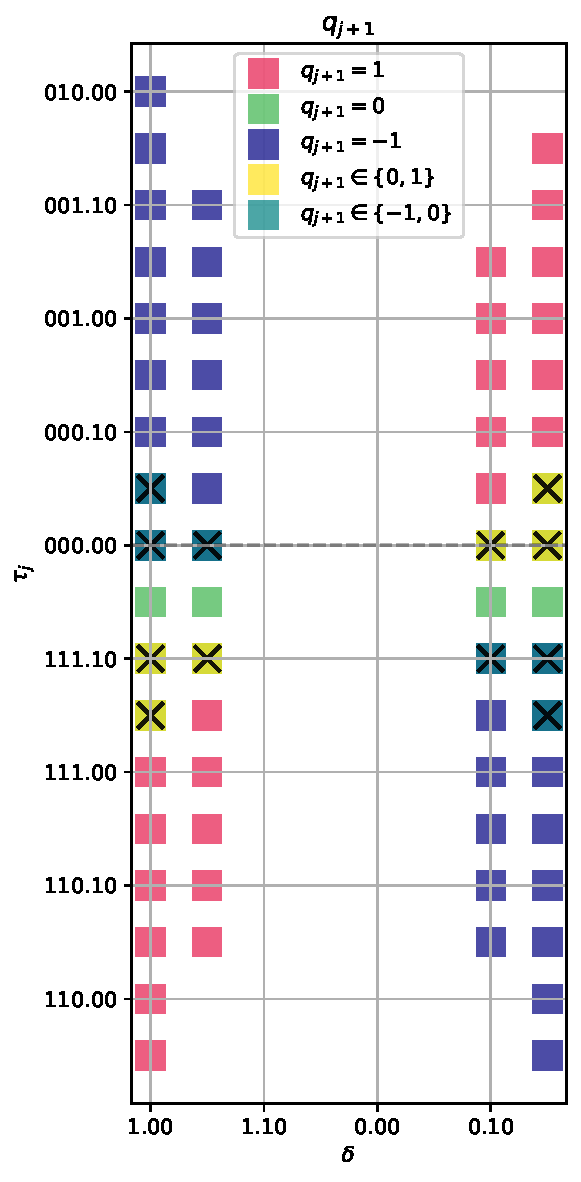
\includegraphics[width=\textwidth, height=3.5\textwidth, keepaspectratio=true]{../figures/division/radix2_qds_basic_quadrants_1_2_3_4.pdf}
    \caption{Radix-2 Basic QDS}
    \label{fig:division:radix2_basic}
  \end{subfigure}
  \hfill
  \begin{subfigure}[b]{0.32\textwidth}
    \centering
    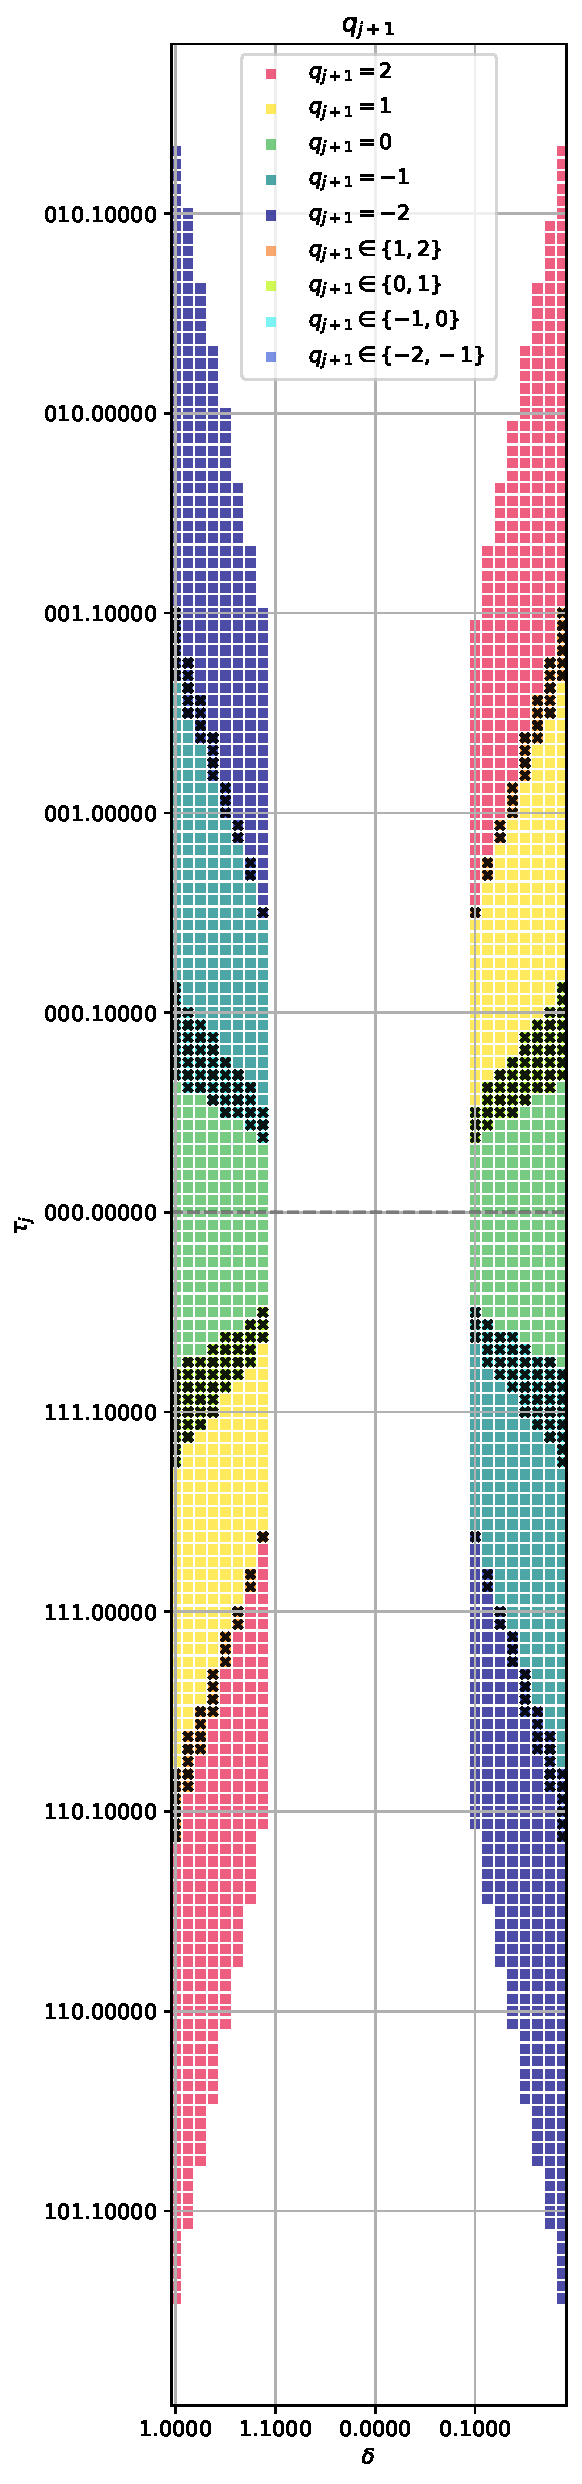
\includegraphics[width=\textwidth, height=3.5\textwidth, keepaspectratio=true]{../figures/division/radix4_qds_basic_quadrants_1_2_3_4.pdf}
    \caption{Radix-4 Basic QDS}
    \label{fig:division:radix4_basic}
  \end{subfigure}
  \hfill
  \begin{subfigure}[b]{0.32\textwidth}
    \centering
    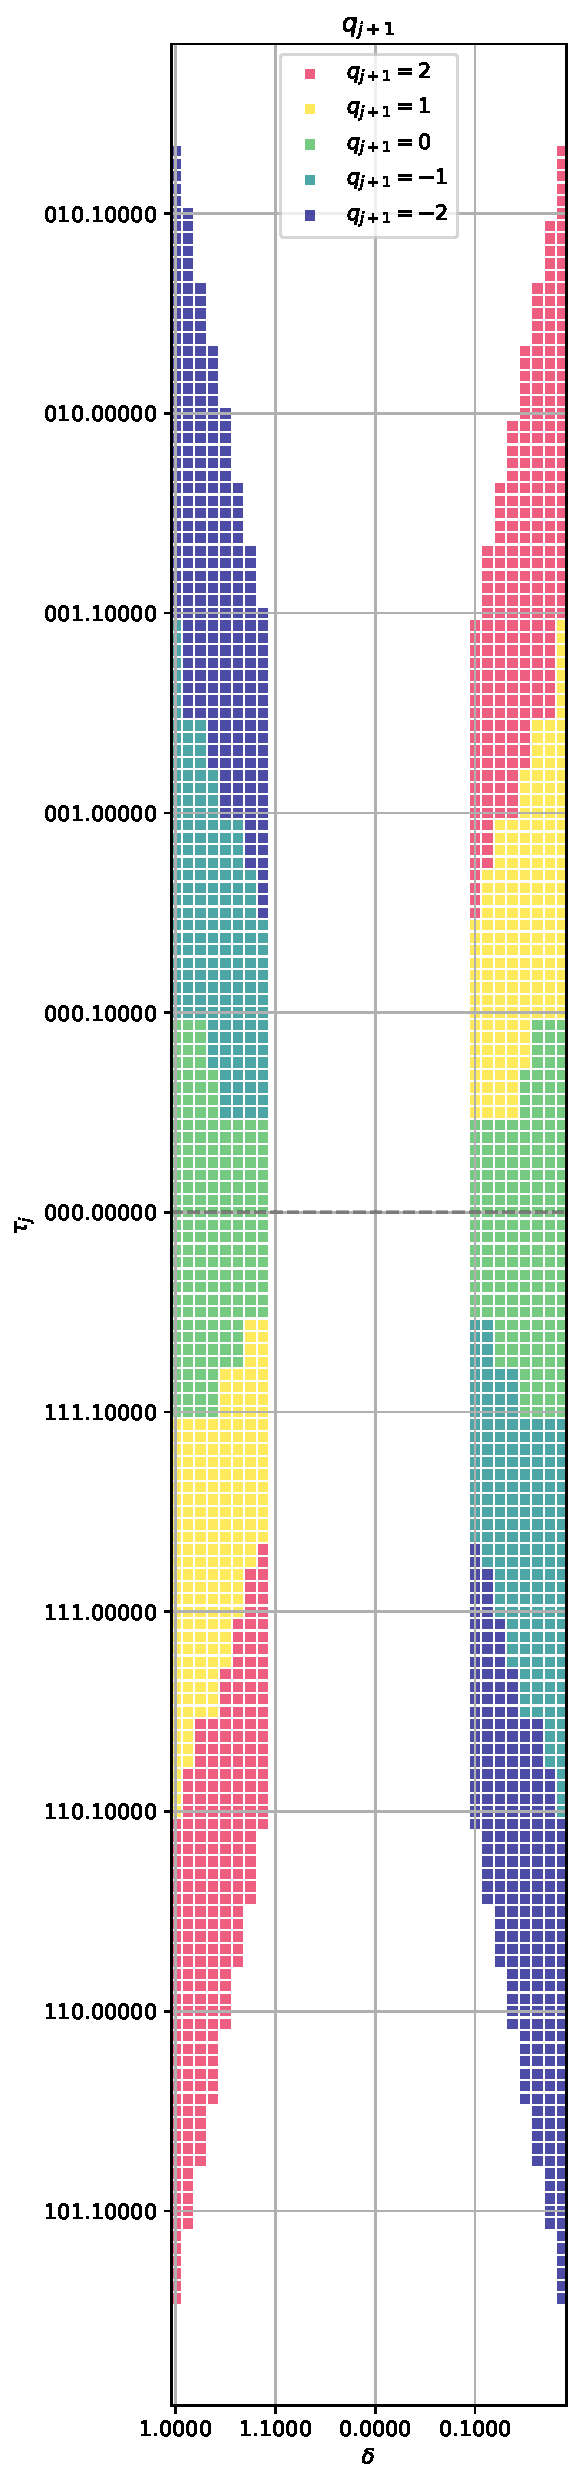
\includegraphics[width=\textwidth, height=3.5\textwidth, keepaspectratio=true]{../figures/division/radix4_qds_optimized_quadrants_1_2_3_4.pdf}
    \caption{Radix-4 Optimized QDS}
    \label{fig:division:radix4_optimized}
  \end{subfigure}
  \caption{Selection regions for the Quotient Digit Selector (QDS). The y-axis is the truncated residual estimate $\tau_j$ and the x-axis is the truncated divisor estimate $\delta$. The plots show how the choice of quotient digit $q_{j+1}$ depends on these estimates.}
  \label{fig:division:qds}
\end{figure}

\section{Square Root by Digit Recurrence}
\label{sec:sqrt}
The digit recurrence methodology can be adapted for square root extraction.
The fundamental relationship is:
\begin{equation}
  \label{eq:sqrt:relation}
  X = S^2 + R
\end{equation}
where $X$ is the radicand, $S$ is the square root, and $R$ is the final remainder.
We again use normalized operands:
\begin{align*}
  X &\in \left[\frac{1}{4}, 1\right) && \text{(Radicand)} \\
  S &\in \left[\sqrt{\frac{1}{4}}, \sqrt{1}\right) = \left[\frac{1}{2}, 1\right) && \text{(Square Root)}
\end{align*}

The root $S$ is computed iteratively for $j = 0, 1, \dots, n-1$.
Let $S_j$ be the root estimate after $j$ digits ($s_1, \dots, s_j$) have been determined.
\begin{equation}
  \label{eq:sqrt:root_recurrence}
  S_{j+1} = S_j + s_{j+1} B^{-(j+1)}
\end{equation}
Unfolding the recurrence:
\begin{equation}
  \label{eq:sqrt:root_unfold}
  \text{At step } j, \quad S_{j+1} = S_0 + \sum_{i=0}^{j} s_{i+1} B^{-(i+1)}
\end{equation}
The final root after $n$ iterations is:
\begin{equation}
  \label{eq:sqrt:root_final}
  \text{At step } j = n-1, \quad S_n = S_0 + \sum_{i=0}^{n-1} s_{i+1} B^{-(i+1)} = S
\end{equation}
The error at step $j$ is $\varepsilon_{j+1} = \sqrt{X} - S_{j+1}$.
As with division, this error is bounded by the maximum possible value of the remaining digits:
\begin{equation}
  \label{eq:sqrt:error_def}
  \varepsilon_{j+1} = \sum_{i=j+1}^{\infty} s_{i+1} B^{-(i+1)}
\end{equation}
\begin{equation}
  \label{eq:sqrt:error_sum}
  \left| \sum_{i=j+1}^{\infty} s_{i+1} B^{-(i+1)} \right| \leq \sum_{i=j+1}^{\infty} a B^{-(i+1)} = a B^{-(j+2)} \sum_{k=0}^{\infty} B^{-k} = a B^{-(j+2)} \frac{1}{1-B^{-1}} = \frac{a}{B-1} B^{-(j+1)}
\end{equation}
This gives the same error bound form as in division:
\begin{equation}
  \label{eq:sqrt:error_bound}
  \left| \varepsilon_{j+1} \right| \leq \rho B^{-(j+1)} \implies \left| \sqrt{X} - S_{j+1} \right| \leq \rho B^{-(j+1)}
\end{equation}
To find the containment condition, we rearrange and square the inequality:
\begin{equation}
  \label{eq:sqrt:error_rearrange}
  S_{j+1} - \rho B^{-(j+1)} \leq \sqrt{X} \leq S_{j+1} + \rho B^{-(j+1)}
\end{equation}
\begin{equation}
  \label{eq:sqrt:error_square}
  S_{j+1}^2 - 2 S_{j+1} \rho B^{-(j+1)} + \rho^2 B^{-2(j+1)} \leq X \leq S_{j+1}^2 + 2 S_{j+1} \rho B^{-(j+1)} + \rho^2 B^{-2(j+1)}
\end{equation}
Isolating the term $X - S_{j+1}^2$:
\begin{equation}
  \label{eq:sqrt:containment_pre}
  \rho^2 B^{-2(j+1)} - 2 S_{j+1} \rho B^{-(j+1)} \leq X - S_{j+1}^2 \leq \rho^2 B^{-2(j+1)} + 2 S_{j+1} \rho B^{-(j+1)}
\end{equation}
We define the scaled residual $R_{j+1} = B^{j+1} (X - S_{j+1}^2)$.
Multiplying by $B^{j+1}$:
\begin{equation}
  \label{eq:sqrt:containment_scaled}
  \rho^2 B^{-(j+1)} - 2 \rho S_{j+1} \leq B^{j+1} (X - S_{j+1}^2) \leq \rho^2 B^{-(j+1)} + 2 \rho S_{j+1}
\end{equation}
This gives the containment condition for the square root residual:
\begin{equation}
  \label{eq:sqrt:containment}
  \rho^2 B^{-(j+1)} - 2 \rho S_{j+1} \leq R_{j+1} \leq \rho^2 B^{-(j+1)} + 2 \rho S_{j+1}
\end{equation}
The final unscaled remainder $R$ is related to the final residual $R_n$ by:
\begin{equation}
  \label{eq:sqrt:final_remainder}
  \text{At step } j = n-1, \quad R_n = B^n (X - S_n^2) = B^n R
\end{equation}
Next, we derive the residual recurrence relation:
\begin{align*}
  R_{j+1} &= B^{j+1} (X - S_{j+1}^2) \\
  &= B^{j+1} \left(X - \left(S_j + s_{j+1} B^{-(j+1)}\right)^2\right) \\
  &= B^{j+1} \left(X - \left(S_j^2 + 2 S_j s_{j+1} B^{-(j+1)} + s_{j+1}^2 B^{-2(j+1)}\right)\right) \\
  &= B^{j+1} (X - S_j^2) - B^{j+1} \left(2 S_j s_{j+1} B^{-(j+1)} + s_{j+1}^2 B^{-2(j+1)}\right) \\
  &= B \left(B^j (X - S_j^2)\right) - \left(2 S_j s_{j+1} + s_{j+1}^2 B^{-(j+1)}\right) \\
  &= B R_j - s_{j+1} \left(2 S_j + s_{j+1} B^{-(j+1)}\right)
\end{align*}
The central recurrence for square root is:
\begin{equation}
  \label{eq:sqrt:residual_recurrence}
  R_{j+1} = B R_j - s_{j+1} \left(2 S_j + s_{j+1} B^{-(j+1)}\right)
\end{equation}
To find the selection intervals, we substitute this recurrence into the containment condition from~\cref{eq:sqrt:containment}:
\begin{equation}
  \label{eq:sqrt:selection_sub1}
  \rho^2 B^{-(j+1)} - 2 \rho S_{j+1} \leq B R_j - s_{j+1} \left(2 S_j + s_{j+1} B^{-(j+1)}\right) \leq \rho^2 B^{-(j+1)} + 2 \rho S_{j+1}
\end{equation}
Substituting $S_{j+1} = S_j + s_{j+1}B^{-(j+1)}$ into the bounds:
\begin{equation}
  \label{eq:sqrt:selection_sub2}
  \rho^2 B^{-(j+1)} - 2 \rho \left(S_j + s_{j+1} B^{-(j+1)}\right) \leq B R_j - s_{j+1} \left(2 S_j + s_{j+1} B^{-(j+1)}\right) \leq \rho^2 B^{-(j+1)} + 2 \rho \left(S_j + s_{j+1} B^{-(j+1)}\right)
\end{equation}
Adding $s_{j+1} \left(2 S_j + s_{j+1} B^{-(j+1)}\right)$ to all parts and simplifying leads to the selection interval for $B R_j$:
\begin{equation}
  \label{eq:sqrt:selection_interval}
  2 (s_{j+1} - \rho) S_j + (s_{j+1} - \rho)^2 B^{-(j+1)} \leq B R_j \leq 2 (s_{j+1} + \rho) S_j + (s_{j+1} + \rho)^2 B^{-(j+1)}
\end{equation}
Unlike division, these bounds depend on the partial result $S_j$, which changes at every step.
This makes the digit selection logic more complex.

\subsection{Initialization}
\label{ssec:sqrt:init}
The first step of the algorithm ($j = 0$) requires initial values for the root approximation, $S_0$, and the residual, $R_0$.
These values must be chosen such that the first shifted residual, $B R_0$, falls within a valid selection region for the first root digit, $s_1$.
This ensures the recurrence can start correctly and that the subsequent residual, $R_1$, will satisfy the containment condition.

A common and robust initialization strategy is to set the initial root approximation to $S_0 = 1$.
While this value is outside the final root's range of $S \in [1/2, 1)$, it is a valid starting point due to the self-correcting nature of the algorithm.
With this choice, the initial residual is defined as:
\begin{equation}
  \label{eq:sqrt:init_r0}
  R_0 = X - S_0^2 = X - 1
\end{equation}
Since the radicand $X$ is in the range $\left[\frac{1}{4}, 1\right)$, the initial residual $R_0$ is always non-positive, with a range of $R_0 \in \left[-\frac{3}{4}, 0\right)$.
A negative residual forces the selection of non-positive digits ($s_k \leq 0$) until the root approximation $S_k$ is brought down into the correct range.

To verify this initialization, we must show that the range of $B R_0$ is fully covered by the union of the selection intervals for $s_1$.
The selection condition for $s_1$ is derived by substituting $j = 0$ and $S_0 = 1$ into the general selection interval formula from \cref{eq:sqrt:selection_interval}:
\begin{equation}
  \label{eq:sqrt:init_selection}
  2(s_1 - \rho) + (s_1 - \rho)^2 B^{-1} \leq B R_0 \leq 2(s_1 + \rho) + (s_1 + \rho)^2 B^{-1}
\end{equation}
Since $B R_0$ is negative, we only need to check the intervals for non-positive digits ($s_1 \in \{0, -1, \dots, -a\}$).

In the Radix-2 case ($B = 2, \rho = 1$), the shifted residual range is $2 R_0 \in \left[-\frac{3}{2}, 0\right)$.
We check the selection intervals for $s_1 = 0$ and $s_1 = -1$:
\begin{itemize}
    \item For $s_1 = 0$: The interval is $[2(0-1) + (0-1)^2 2^{-1}, 2(0+1) + (0+1)^2 2^{-1}] = [-1.5, 2.5]$.
    \item For $s_1 = -1$: The interval is $[2(-1-1) + (-1-1)^2 2^{-1}, 2(-1+1) + (-1+1)^2 2^{-1}] = [-2, 0]$.
\end{itemize}
The union of these intervals covers the range $[-2, 2.5]$, which safely contains the required range of $2 R_0 \in [-1.5, 0)$.
Thus, the initialization is valid.

In the Radix-4 case ($B = 4, \rho = 2/3$), the shifted residual range is $4 R_0 \in [-3, 0)$.
We check the intervals for $s_1 \in \{0, -1, -2\}$:
\begin{itemize}
    \item For $s_1 = 0$: The interval is $\left[2\left(0-\frac{2}{3}\right) + \left(0-\frac{2}{3}\right)^2 4^{-1}, 2\left(0+\frac{2}{3}\right) + \left(0+\frac{2}{3}\right)^2 4^{-1}\right] = \left[-\frac{4}{3} + \frac{1}{9}, \frac{4}{3} + \frac{1}{9}\right] \approx [-1.22, 1.44]$.
    \item For $s_1 = -1$: The interval is $\left[2\left(-1-\frac{2}{3}\right) + \left(-1-\frac{2}{3}\right)^2 4^{-1}, 2\left(-1+\frac{2}{3}\right) + \left(-1+\frac{2}{3}\right)^2 4^{-1}\right] = \left[-\frac{10}{3} + \frac{25}{36}, -\frac{2}{3} + \frac{1}{36}\right] \approx [-2.64, -0.64]$.
    \item For $s_1 = -2$: The interval is $\left[2\left(-2-\frac{2}{3}\right) + \left(-2-\frac{2}{3}\right)^2 4^{-1}, 2\left(-2+\frac{2}{3}\right) + \left(-2+\frac{2}{3}\right)^2 4^{-1}\right] = \left[-\frac{16}{3} + \frac{16}{9}, -\frac{8}{3} + \frac{4}{9}\right] \approx [-3.56, -2.22]$.
\end{itemize}
The union of these intervals covers the range $[-3.56, 1.44]$, which safely contains the required range of $4 R_0 \in [-3, 0)$.
This confirms the initialization is also valid for the Radix-4 case.

\subsection{Example: Radix-2 SRT Square Root}
\label{ssec:sqrt:radix2}
We use $B = 2$, $a = 1$, so $\rho = 1$.
The digit set for $s_{j+1}$ is $\{-1, 0, 1\}$.
The selection intervals from~\cref{eq:sqrt:selection_interval} become:
\begin{equation}
  \label{eq:sqrt:radix2_intervals}
  s_{j+1} =
  \begin{cases}
    1  & \text{if } 0 \leq 2 R_j \leq 4 S_j + 4 \cdot 2^{-(j+1)} \\
    0  & \text{if } -2 S_j + 2^{-(j+1)} \leq 2 R_j \leq 2 S_j + 2^{-(j+1)} \\
    -1 & \text{if } -4 S_j + 4 \cdot 2^{-(j+1)} \leq 2 R_j \leq 0
  \end{cases}
\end{equation}
The selection depends on both the shifted residual $2R_j$ and the partial root $S_j$.
We need truncated estimates of both.
The residual $2 R_j = r_{j,3\ldots0}.r_{j,-1\ldots-\infty}$ is handled as before, with a truncated estimate $t_j$ having an error $0 \leq 2 R_j - t_j < 2^{-(\alpha-1)}$.
The integer estimates are:
\begin{align}
  \label{eq:sqrt:radix2_tau_def}
  \tau_j &= \Int(2^\alpha \cdot t_{j,3\ldots0}.t_{j,-1\ldots-\alpha}) \in \left\{-2^{\alpha+3}, \dots, 2^{\alpha+3}-1\right\} && (\tau_j \leq 2^{\alpha+1} R_j < \tau_j + 2) \\
  \label{eq:sqrt:radix2_sigma_def}
  \sigma_j &= \Int(2^\beta \cdot 0.1s_{j,-2\ldots-\beta}) \in \left\{2^{\beta-1}, \dots, 2^\beta-1\right\} && (\sigma_j \leq 2^\beta S_j \leq \sigma_j + 1 - 2^\beta \mathrm{ulp})
\end{align}
The partial root $S_j$ is in the range $[1/2, 1)$, and its ulp (unit in the last place) is $2^{-j}$.
So the bound on the estimate is $\sigma_j \leq 2^\beta S_j \leq \sigma_j + 1 - 2^\beta 2^{-j}$.

The continuity condition analysis is more complex than for division.
Let $L_k(S_j)$ and $U_k(S_j)$ be the lower and upper bounds from~\cref{eq:sqrt:selection_interval}.
The condition is $\min(U_{k-1,\mathrm{trunc}}) \geq \max(L_{k,\mathrm{trunc}})$.
With $\rho = 1, B = 2$:
\begin{itemize}
  \item For $k = 1$: $\min(U_{0,\mathrm{trunc}}) \geq \max(L_{1,\mathrm{trunc}})$. This gives $2 \cdot 2^{-\beta} \sigma_j - 2^{-(\alpha-1)} \geq 0$. This holds for $\alpha \geq 1$ since $\sigma_j \geq 2^{\beta-1}$.
  \item For $k = 0$: $\min(U_{-1,\mathrm{trunc}}) \geq \max(L_{0,\mathrm{trunc}})$. This gives $2 \cdot 2^{-\beta} \sigma_j - 2^{-(\alpha-1)} - B^{-(j+1)} \geq 0$.
\end{itemize}
The condition for $k = 0$ is more restrictive due to the $-B^{-(j+1)}$ term.
For the worst case (smallest $\sigma_j = 2^{\beta-1}$), we need $2 \cdot 2^{-\beta} (2^{\beta-1}) - 2^{-(\alpha-1)} - 2^{-(j+1)} = 1 - 2^{-(\alpha-1)} - 2^{-(j+1)} \geq 0$.
This requires $\alpha \geq 2$.
Choosing $\alpha = 2, \beta = 2$:
\begin{align}
  \label{eq:sqrt:radix2_tau_val}
  \tau_j &= \Int(4 \cdot t_{j,3\ldots0}.t_{j,-1}t_{j,-2}) \in \left\{-32, \dots, 31\right\} && (\tau_j \leq 8 R_j < \tau_j + 2) \\
  \label{eq:sqrt:radix2_sigma_val}
  \sigma_j &= \Int(4 \cdot 0.1s_{j,-2}) \in \left\{2, 3\right\} && (\sigma_j \leq 4 S_j \leq \sigma_j + 1 - 4 \cdot 2^{-j})
\end{align}
The selection logic becomes:
\begin{equation}
  \label{eq:sqrt:radix2_logic}
  s_{j+1} =
  \begin{cases}
    1  & \text{if } 0 \leq \tau_j < 4 (\sigma_j + 1) \\
    0  & \text{if } -2 (\sigma_j - 1) \leq \tau_j \leq 2 \sigma_j - 2 \\
    -1 & \text{if } -4 (\sigma_j + 1) - 2 < \tau_j \leq -2
  \end{cases}
\end{equation}

\subsubsection{Special Case: Radicand Close to 1}
\label{sssec:sqrt:radix2_special}
A special condition arises in the initial iterations of the square root algorithm if the first few selected digits are zero.
If $s_1, \dots, s_j$ are all 0, the partial root $S_j$ remains at its initial value, $S_j = S_0 = 1$.
This simplifies the selection logic, as the partial root estimate $\sigma_j$ becomes a constant.
This scenario is particularly relevant for radicands $X$ that are close to 1.

For the Radix-2 case, we use precision parameters $\alpha = 2$ and $\beta = 2$.
The integer estimate of the scaled residual $2 R_j$ is $\tau_j$.
Since the initial residual $R_0 = X - 1$ is negative, and the recurrence simplifies to $R_k = B R_{k-1}$ when $s_k = 0$, the residual $R_j$ remains negative as long as only zero-digits are selected, making its estimate $\tau_j$ also negative.
The integer estimate of the scaled partial root $S_j$ is $\sigma_j$.
Since $S_j = 1$, its value is constant.
\begin{align}
  \label{eq:sqrt:radix2_tau_special}
  \tau_j &= \Int(4 \cdot 1t_{j,2\ldots0}.t_{j,-1}t_{j,-2}) \in \left\{-32, \dots, -1\right\} && (\tau_j \leq 8 R_j < \tau_j + 2) \\
  \label{eq:sqrt:radix2_sigma_special}
  \sigma_j &= \Int(4 \cdot 1.00) = 4 && (4 S_j = \sigma_j)
\end{align}
The selection logic becomes:
\begin{equation}
  \label{eq:sqrt:radix2_logic_special}
  s_{j+1} =
  \begin{cases}
    0  & \text{if } -2 (\sigma_j - 1) \leq \tau_j \leq -1 \\
    -1 & \text{if } -4 \sigma_j - 2 < \tau_j \leq -2
  \end{cases}
\end{equation}

\subsection{Example: Radix-4 SRT Square Root}
\label{ssec:sqrt:radix4}
We use $B = 4$, $a = 2$, so $\rho = 2/3$.
The digit set for $s_{j+1}$ is $\{-2, \dots, 2\}$.
The selection intervals from~\cref{eq:sqrt:selection_interval} are:
\begin{equation}
  \label{eq:sqrt:radix4_intervals}
  s_{j+1} =
  \begin{cases}
    2  & \text{if } \frac{8}{3} S_j + \frac{16}{9} 4^{-(j+1)} \leq 4 R_j \leq \frac{16}{3} S_j + \frac{64}{9} 4^{-(j+1)} \\
    1  & \text{if } \frac{2}{3} S_j + \frac{1}{9} 4^{-(j+1)} \leq 4 R_j \leq \frac{10}{3} S_j + \frac{25}{9} 4^{-(j+1)} \\
    0  & \text{if } -\frac{4}{3} S_j + \frac{4}{9} 4^{-(j+1)} \leq 4 R_j \leq \frac{4}{3} S_j + \frac{4}{9} 4^{-(j+1)} \\
    -1 & \text{if } -\frac{10}{3} S_j + \frac{25}{9} 4^{-(j+1)} \leq 4 R_j \leq -\frac{2}{3} S_j + \frac{1}{9} 4^{-(j+1)} \\
    -2 & \text{if } -\frac{16}{3} S_j + \frac{64}{9} 4^{-(j+1)} \leq 4 R_j \leq -\frac{8}{3} S_j + \frac{16}{9} 4^{-(j+1)}
  \end{cases}
\end{equation}
The integer estimates are:
\begin{align}
  \label{eq:sqrt:radix4_tau_def}
  \tau_j &= \Int(2^\alpha \cdot t_{j,3\ldots0}.t_{j,-1\ldots-\alpha}) \in \left\{-2^{\alpha+3}, \dots, 2^{\alpha+3}-1\right\} && (\tau_j \leq 2^{\alpha+2} R_j < \tau_j + 2) \\
  \label{eq:sqrt:radix4_sigma_def}
  \sigma_j &= \Int(2^\beta \cdot 0.1s_{j,-2\ldots-\beta}) \in \left\{2^{\beta-1}, \dots, 2^\beta-1\right\} && (\sigma_j \leq 2^\beta S_j \leq \sigma_j + 1 - 2^\beta 4^{-j})
\end{align}
The continuity condition $\min(U_{k-1,\mathrm{trunc}}) \geq \max(L_{k,\mathrm{trunc}})$ must hold for $k \in \{-1, 0, 1, 2\}$.
Substituting $\rho = 2/3$ and simplifying gives the conditions:
\begin{itemize}
  \item For $k = 2$: $\frac{2}{3} \cdot 2^{-\beta} \sigma_j - \frac{8}{3} \cdot 2^{-\beta} - 2^{-(\alpha-1)} \geq 0$.
  \item For $k = 1$: $\frac{2}{3} \cdot 2^{-\beta} \sigma_j - \frac{2}{3} \cdot 2^{-\beta} - 2^{-(\alpha-1)} \geq 0$.
  \item For $k = 0$: $\frac{2}{3} \cdot 2^{-\beta} \sigma_j - \frac{2}{3} \cdot 2^{-\beta} - 2^{-(\alpha-1)} - \frac{4}{9} B^{-(j+1)} \geq 0$.
  \item For $k = -1$: $\frac{2}{3} \cdot 2^{-\beta} \sigma_j - \frac{8}{3} \cdot 2^{-\beta} - 2^{-(\alpha-1)} - \frac{25}{9} B^{-(j+1)} \geq 0$.
\end{itemize}
A significant complication arises in the continuity analysis for square root that is not present in division.
The selection bounds in~\cref{eq:sqrt:selection_interval} contain terms proportional to $B^{-(j+1)}$, originating from the $(s_{j+1} \pm \rho)^2$ components.
These terms cause the overlap between selection regions to depend on the iteration number $j$.
Consequently, the available overlap can shrink, making the digit selection more difficult.
This problem is most acute for early iterations (small $j$) where the $B^{-(j+1)}$ factor is largest, and for negative choices of the digit $k$ where the $(k \pm \rho)^2$ coefficients are largest.
The most restrictive case is the boundary between selecting $k = -1$ and $k = -2$.
For this boundary, the continuity condition becomes:
\[
  \frac{2}{3} \cdot 2^{-\beta} \sigma_j - \frac{8}{3} \cdot 2^{-\beta} - 2^{-(\alpha-1)} - \frac{25}{9} B^{-(j+1)} \geq 0.
\]
This inequality must hold for the selection logic to be valid, but the final term may cause it to fail for small values of $j$.
For instance, with parameters $\alpha = 4, \beta = 4$, radix $B = 4$, and a worst-case partial root estimate ($\sigma_j = 8$), the constant part of the inequality is $\frac{1}{24}$.
The condition simplifies to:
\[
  \frac{1}{24} - \frac{25}{9} 4^{-(j+1)} \geq 0.
\]
This is only met for $j \geq 3$.
The failure for the initial iterations ($j = 0, 1, 2$) means they require a more precise selection mechanism or a special startup sequence.
For $j \geq 3$, we can use the parameters $\alpha = 4, \beta = 4$:
\begin{align}
  \label{eq:sqrt:radix4_tau_val}
  \tau_j &= \Int(16 \cdot t_{j,3\ldots0}.t_{j,-1\ldots-4}) \in \left\{-128, \dots, 127\right\} && (\tau_j \leq 64 R_j < \tau_j + 2) \\
  \label{eq:sqrt:radix4_sigma_val}
  \sigma_j &= \Int(16 \cdot 0.1s_{j,-2\ldots-4}) \in \left\{8, \dots, 15\right\} && (\sigma_j \leq 16 S_j \leq \sigma_j + 1 - 16 \cdot 4^{-j})
\end{align}
The selection logic for $j \geq 3$ is:
\begin{equation}
  \label{eq:sqrt:radix4_logic}
  s_{j+1} =
  \begin{cases}
    2  & \text{if } \frac{8}{3} (\sigma_j + 1) \leq \tau_j < \frac{16}{3} (\sigma_j + 1) \\
    1  & \text{if } \frac{2}{3} (\sigma_j + 1) \leq \tau_j \leq \frac{10}{3} \sigma_j - 2 \\
    0  & \text{if } -\frac{4}{3} \left(\sigma_j - \frac{1}{48}\right) \leq \tau_j \leq \frac{4}{3} \sigma_j - 2 \\
    -1 & \text{if } -\frac{10}{3} \left(\sigma_j - \frac{5}{96}\right) \leq \tau_j \leq -\frac{2}{3} (\sigma_j + 1) - 2 \\
    -2 & \text{if } -\frac{16}{3} (\sigma_j + 1) - 2 < \tau_j \leq -\frac{8}{3} (\sigma_j + 1) - 2
  \end{cases}
\end{equation}

\subsubsection{Startup Issues and Iteration-Dependent Selection}
\label{sssec:sqrt:radix4_special}
As with the Radix-2 case, we can analyze the special condition where $s_1, \dots, s_j = 0$, which implies $S_j = 1$.
However, the analysis reveals a complication: the validity of the selection logic becomes dependent on the iteration index $j$.

The most restrictive continuity condition for Radix-4 square root is for selecting between $s_{j+1} = -1$ and $s_{j+1} = -2$.
As derived previously, this condition is:
\begin{equation*}
  \frac{2}{3} \cdot 2^{-\beta} \sigma_j - \frac{8}{3} \cdot 2^{-\beta} - 2^{-(\alpha-1)} - \frac{25}{9} B^{-(j+1)} \geq 0
\end{equation*}
Let's test this inequality for our special case, substituting $B = 4$, $\alpha = 4$, $\beta = 4$, and the constant value $\sigma_j = 16$:
\begin{align*}
  \frac{2}{3} \cdot 2^{-4} (16) - \frac{8}{3} \cdot 2^{-4} - 2^{-(4-1)} - \frac{25}{9} 4^{-(j+1)} &\geq 0 \\
  \frac{2}{3} - \frac{1}{6} - \frac{1}{8} - \frac{25}{9} 4^{-(j+1)} &\geq 0 \\
  \frac{3}{8} - \frac{25}{9} 4^{-(j+1)} &\geq 0
\end{align*}
This final inequality must hold for the selection logic to be valid.
However, it clearly depends on $j$.
\begin{itemize}
  \item For $j = 0$: $\frac{3}{8} - \frac{25}{9 \cdot 4} = \frac{3}{8} - \frac{25}{36} = \frac{27 - 50}{72} = -\frac{23}{72} \ngeq 0$. The condition fails.
  \item For $j = 1$: $\frac{3}{8} - \frac{25}{9 \cdot 16} = \frac{3}{8} - \frac{25}{144} = \frac{54 - 25}{144} = \frac{29}{144} \geq 0$. The condition holds.
\end{itemize}
This demonstrates that the standard selection logic is not guaranteed to work for the first iteration, necessitating a special, more precise startup mechanism.
For $j \geq 1$, we can use the parameters $\alpha = 4, \beta = 4$:
\begin{align}
  \label{eq:sqrt:radix4_tau_special}
  \tau_j &= \Int(16 \cdot 1t_{j,2\ldots0}.t_{j,-1\ldots-4}) \in \left\{-128, \dots, -1\right\} && (\tau_j \leq 64 R_j < \tau_j + 2) \\
  \label{eq:sqrt:radix4_sigma_special}
  \sigma_j &= \Int(16 \cdot 1.0000) = 16 && (16 S_j = \sigma_j)
\end{align}
The selection logic for $j \geq 1$ is:
\begin{equation}
  \label{eq:sqrt:radix4_logic_special}
  s_{j+1} =
  \begin{cases}
    0  & \text{if } -\frac{4}{3} \left(\sigma_j - \frac{1}{3}\right) \leq \tau_j \leq -1 \\
    -1 & \text{if } -\frac{10}{3} \left(\sigma_j - \frac{5}{6}\right) \leq \tau_j \leq -\frac{2}{3} \sigma_j - 2 \\
    -2 & \text{if } -\frac{16}{3} \sigma_j - 2 < \tau_j \leq -\frac{8}{3} \sigma_j - 2
  \end{cases}
\end{equation}

\begin{figure}[htbp]
  \centering
  \begin{subfigure}[b]{0.32\textwidth}
    \centering
    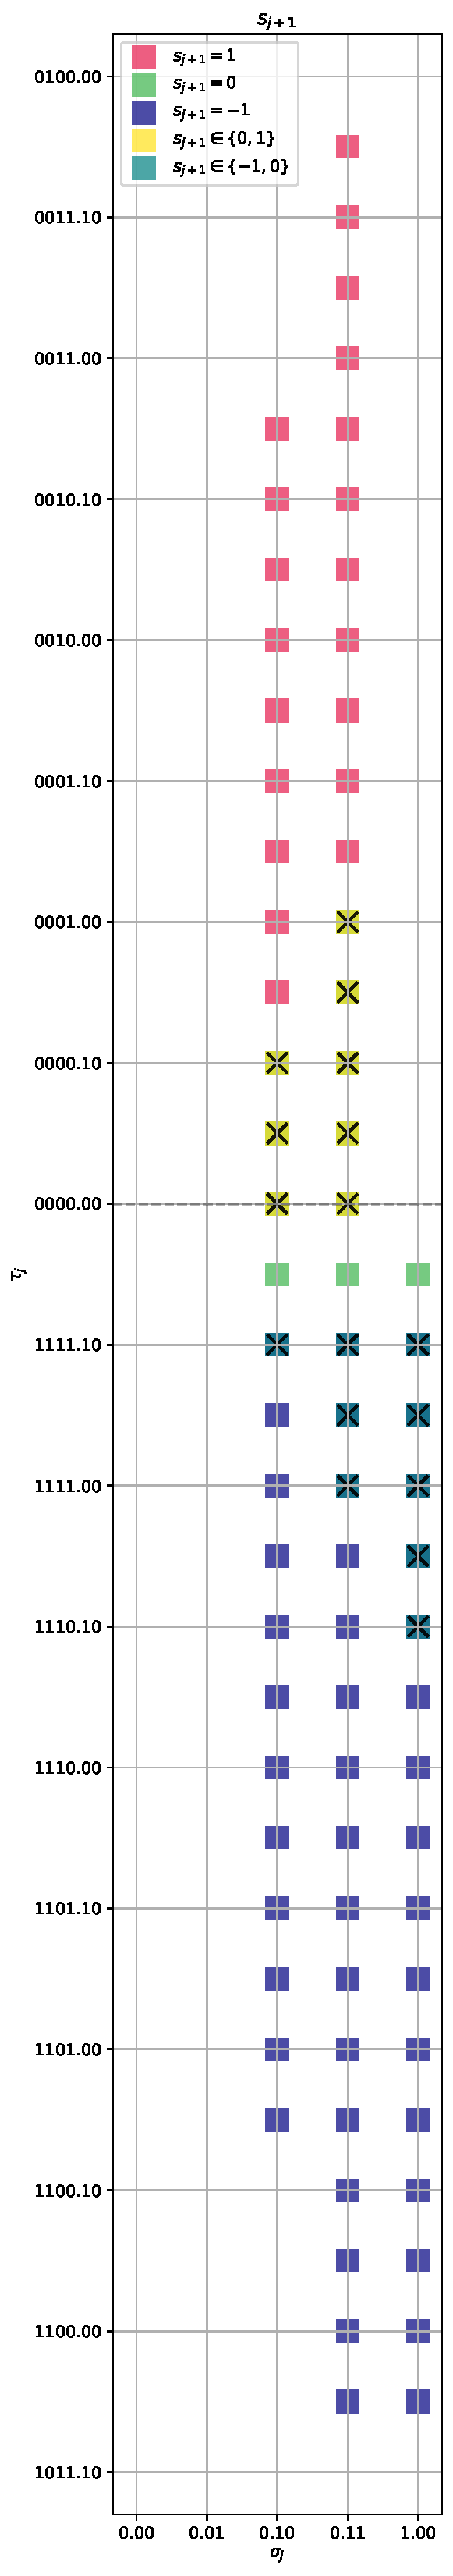
\includegraphics[width=\textwidth, height=3.5\textwidth, keepaspectratio=true]{../figures/square_root/radix2_rds_basic_quadrants_1_4.pdf}
    \caption{Radix-2 Basic RDS}
    \label{fig:sqrt:radix2_basic}
  \end{subfigure}
  \hfill
  \begin{subfigure}[b]{0.32\textwidth}
    \centering
    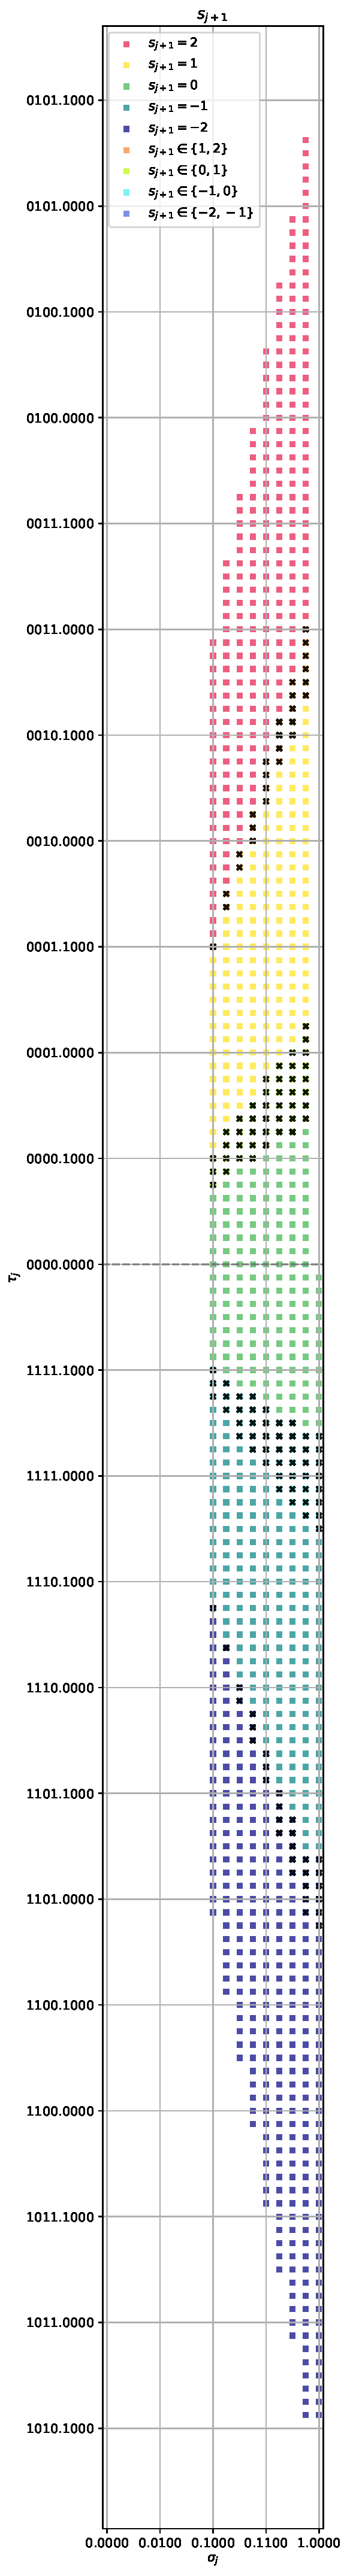
\includegraphics[width=\textwidth, height=3.5\textwidth, keepaspectratio=true]{../figures/square_root/radix4_rds_basic_quadrants_1_4.pdf}
    \caption{Radix-4 Basic RDS}
    \label{fig:sqrt:radix4_basic}
  \end{subfigure}
  \hfill
  \begin{subfigure}[b]{0.32\textwidth}
    \centering
    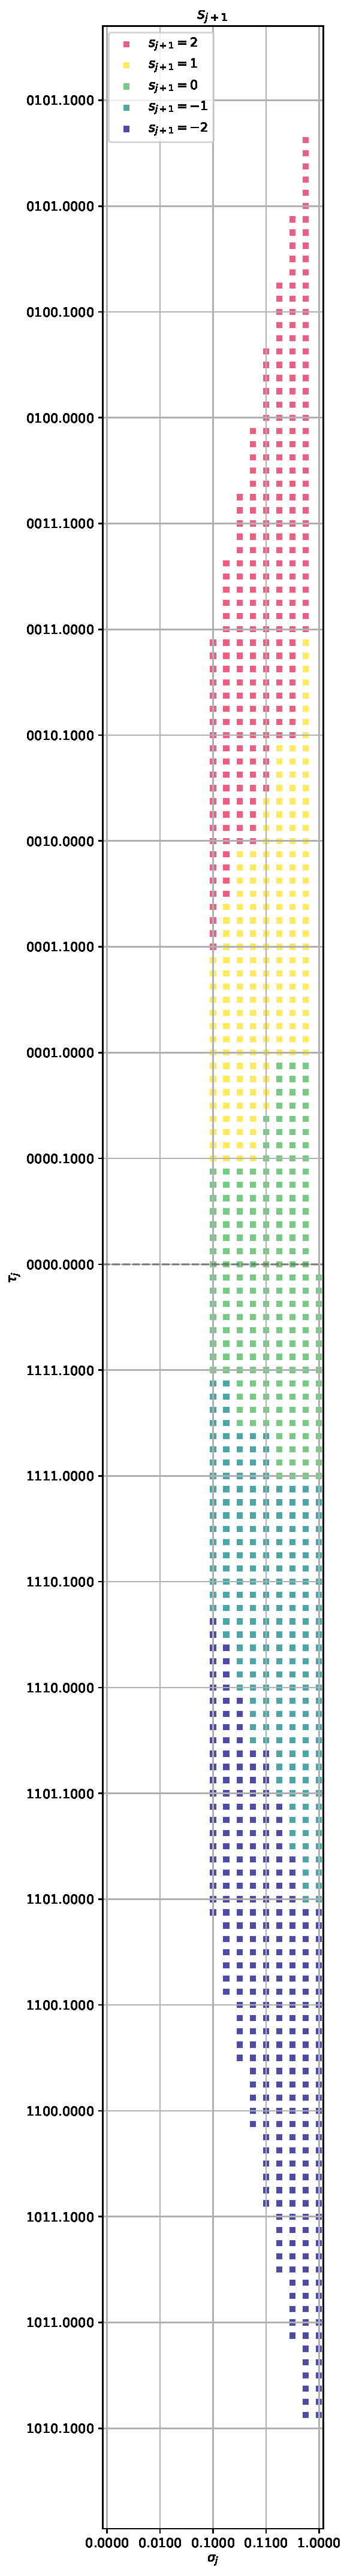
\includegraphics[width=\textwidth, height=3.5\textwidth, keepaspectratio=true]{../figures/square_root/radix4_rds_optimized_quadrants_1_4.pdf}
    \caption{Radix-4 Optimized RDS}
    \label{fig:sqrt:radix4_optimized}
  \end{subfigure}
  \caption{Selection regions for the Root Digit Selector (RDS). The y-axis is the truncated residual estimate $\tau_j$ and the x-axis is the truncated partial root estimate $\sigma_j$. The plots show how the choice of root digit $s_{j+1}$ depends on these estimates.}
  \label{fig:sqrt:rds}
\end{figure}

\begin{table}[htbp]
  \centering
  \caption{Example selection logic constants for a Radix-4 implementation. The table shows the required integer range for the truncated residual estimate $\tau_j$ to select a given digit, based on the truncated divisor/root estimate ($\delta$ or $\sigma_j$).}
  \label{tab:radix4-logic-example}
  \begin{tabular}{@{}lccccc@{}}
    \toprule
    \textbf{$\tau_j$} & \textbf{$q_{j+1}, s_{j+1} = 2$} & \textbf{$q_{j+1}, s_{j+1} = 1$} & \textbf{$q_{j+1}, s_{j+1} = 0$} & \textbf{$q_{j+1}, s_{j+1} = -1$} & \textbf{$q_{j+1}, s_{j+1} = -2$} \\
    \midrule
    $\delta, \sigma_j = 8$  & 24 to 49               & 8 to 23                & -8 to 7                & -26 to -9               & -50 to -27              \\
    $\delta, \sigma_j = 9$  & 28 to 53               & 8 to 27                & -8 to 7                & -28 to -9               & -56 to -29              \\
    $\delta, \sigma_j = 10$ & 32 to 59               & 8 to 31                & -12 to 7               & -32 to -13              & -60 to -33              \\
    $\delta, \sigma_j = 11$ & 32 to 65               & 8 to 31                & -12 to 7               & -34 to -13              & -66 to -35              \\
    $\delta, \sigma_j = 12$ & 36 to 71               & 12 to 35               & -12 to 11              & -36 to -13              & -72 to -37              \\
    $\delta, \sigma_j = 13$ & 40 to 75               & 16 to 39               & -16 to 15              & -40 to -17              & -76 to -41              \\
    $\delta, \sigma_j = 14$ & 40 to 81               & 16 to 39               & -16 to 15              & -44 to -17              & -82 to -45              \\
    $\delta, \sigma_j = 15$ & 48 to 85               & 16 to 47               & -16 to 15              & -48 to -17              & -88 to -49              \\
    \bottomrule
  \end{tabular}
\end{table}

\section{Conclusion}
\label{sec:conclusion}
Digit recurrence algorithms provide an elegant and efficient framework for implementing division and square root in hardware.
They resolve a fundamental conflict at the heart of iterative arithmetic: the need for high precision in the critical path inherently limits speed.
As this tutorial has demonstrated, the core principle of redundancy elegantly resolves this conflict.
By employing a redundant digit set for the result, characterized by a redundancy factor $\rho > 1/2$, these algorithms create overlapping selection regions.
This overlap is the key that unlocks high performance, as it permits the critical selection of the next result digit to be based on fast, low-precision estimates of the internal state.

We have systematically derived the fundamental recurrence relations and shown how the theoretical guarantee of redundancy is translated into a practical hardware implementation.
The continuity condition serves as the crucial bridge, providing a rigorous method to determine the minimum required precision for the truncated operands.
This analysis ensures that the uncertainty introduced by truncation is always less than the overlap provided by redundancy, guaranteeing a correct choice can always be made.
The journey from the abstract recurrence relations to the concrete selection logic tables for Radix-2 and Radix-4 illustrates a complete and robust design methodology.

The power of this methodology was shown to extend from the relatively straightforward case of division, with its static divisor $D$, to the more intricate square root operation.
The latter's reliance on a dynamic, evolving partial root $S_j$ introduces greater complexity, particularly for higher-radix designs.
As we saw in the Radix-4 square root example, iteration-dependent terms can shrink the available overlap, demanding higher precision or special startup logic.
This highlights the inherent trade-offs between performance (radix), complexity, and area that designers must navigate.

Ultimately, digit recurrence methods exemplify a powerful design paradigm where algorithmic properties are exploited to optimize hardware performance.
By trading the simplicity of a non-redundant number system for the flexibility of redundancy, they break the performance bottleneck of traditional iterative approaches.
They are not merely a topic of academic interest but form the foundation of essential, high-performance arithmetic units in virtually all modern processors, standing as a cornerstone of practical computer arithmetic.

\end{document}
